\documentclass[12pt]{article}
\usepackage[margin=1in]{geometry}
\usepackage{fancyvrb}
\usepackage{multicol}

\usepackage[listings]{tcolorbox}

\definecolor{codegreen}{rgb}{0,0.6,0}
\definecolor{codegray}{rgb}{0.5,0.5,0.5}
\definecolor{codepurple}{rgb}{0.58,0,0.82}
\definecolor{backcolour}{rgb}{0.95,0.95,0.92}

\lstdefinestyle{mystyle}{
    language=Python,
    backgroundcolor=\color{backcolour},   
    commentstyle=\color{codegreen},
    keywordstyle=\color{magenta},
    numberstyle=\tiny\color{codegray},
    stringstyle=\color{codepurple},
    basicstyle=\ttfamily\footnotesize,
    breakatwhitespace=false,         
    breaklines=true,                 
    captionpos=b,                    
    keepspaces=true,                 
    numbers=left,                    
    numbersep=5pt,                  
    showspaces=false,                
    showstringspaces=false,
    showtabs=false,                  
    tabsize=2,
    escapechar=|,
    frame=single
}

\lstset{style=mystyle}
\begin{document}
\sloppy
\centerline{\Large CSCI 111, Lab 3}
\centerline{\large Geoffrey Matthews}

\begin{description}
\item[Due date:] Midnight, Tuesday, September 27, on Canvas.
No late work accepted.  

\item[File names:]  Names of files and variables, when specified,
must be EXACTLY as specified.  This includes simple mistakes such
as capitalization.

\item[Individual work:]  All work must be your own.  Do not share
code with anyone other than the instructor and teaching assistants.
This includes looking over shoulders at screens with the code open.
You may discuss ideas, algorithms, approaches, {\em etc.} with
other students but NEVER actual code.

\item[grid:] 
I wrote four solutions to the grid problem from the text,
Chapter 3, Exercise 3.  These files are available on github.com/geofmatthews/csci111
in the folder with the lecture notes for chapter 3, and called {\tt grid00.py,
grid01.py, grid02.py,} and {\tt grid03.py}.

Modify each of these files so that they make a 4x4 grid of squares
instead of a $2x2$ grid.  Make as few changes to the files as you can.

Each line that is modified from the original should have a comment
at the end of the line like this:
\begin{verbatim}
x = func(y)                # CHANGED
\end{verbatim}
Each line that is new  and not in the original should have a comment
at the end of the line like this:
\begin{verbatim}
x = func(y)                  # NEW
\end{verbatim}

Leave the filenames as {\tt grid00.py}, {\em etc.}



\item[Minkowski islands:]  Do Exercise 6, Chapter 5, in the textbook 
on the Koch curve and the Koch snowflake.  Feel free to look at
the author's solutions after you have done it yourself.  You do NOT
have to turn in your snowflake.

\begin{itemize}
\item Look up {\bf Minkowski sausage} in Wikipedia.  There
you will find three generators for Minkowski sausages, illustrated
in Figures \ref{kochtype1}, \ref{kochtype2}, and \ref{kochtype16}.


\item Each of these can be used to make a {\bf Minkowski Island}
by drawing four of them around a square.

\item Write a function for each of these generators, and 
place each in its own file: 
\begin{description}\tt
\item koch1 {\rm in} koch1.py
\item koch2 {\rm in} koch2.py
\item koch15 {\rm in} koch16.py
\end{description}

\item Each function will take as arguments a turtle and a distance,
as in the {\tt snowflake} solution accompanying the textbook.

\item The recursion is stopped when the distance is less than 10.

\item Each generator uses a different reduction in size
for the distance in the recursive calls.  Figure out which
distance will preserve the total length, regardless of how big
it is.

\item Write a single function {\tt island}, that takes a turtle
and a generator as arguments, and makes the turtle draw
the generator around all four sides of a square.
Islands look like Figures  \ref{kochtype1island},
\ref{kochtype2island}, and \ref{kochtype16island}.

\item In each of your three files, define a turtle {\tt bob},
set its speed to 0, and call {\tt island(bob, 200, {\sl generator})} so that
the island will be drawn when the module is run.

\item
Replace {\sl generator} in each case with {\tt koch1}, {\tt koch2}
or {\tt koch16}, accordingly.

\begin{figure}[!htbp]
\centerline{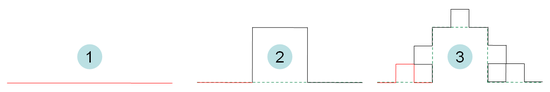
\includegraphics[width=0.75\textwidth]{kochtype1}}
\caption{Koch type 1 generator}
\label{kochtype1}
\end{figure}

\begin{figure}[!htbp]
\centerline{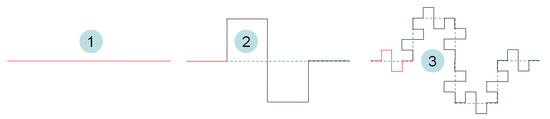
\includegraphics[width=0.75\textwidth]{kochtype2}}
\caption{Koch type 2 generator}
\label{kochtype2}
\end{figure}

\begin{figure}[!htbp]
\centerline{
\includegraphics[width=0.75\textwidth]{kochtype16} }
\caption{Koch type 1.6 generator}
\label{kochtype16}
\end{figure}

\begin{figure}[!htbp]
\centerline{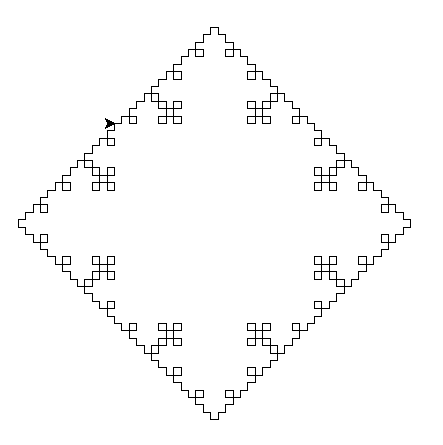
\includegraphics[width=0.333\textwidth]{kochtype1island} }
\caption{Koch type 1 island}
\label{kochtype1island}
\end{figure}
\begin{figure}[!htbp]
\centerline{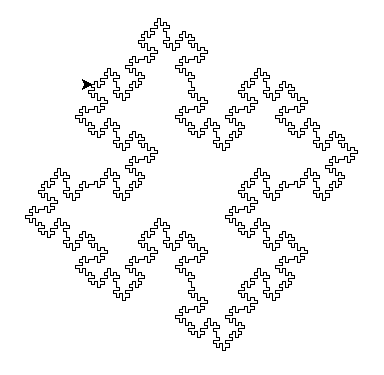
\includegraphics[width=0.333\textwidth]{kochtype2island} }
\caption{Koch type 2 island}
\label{kochtype2island}
\end{figure}
\begin{figure}[!htbp]
\centerline{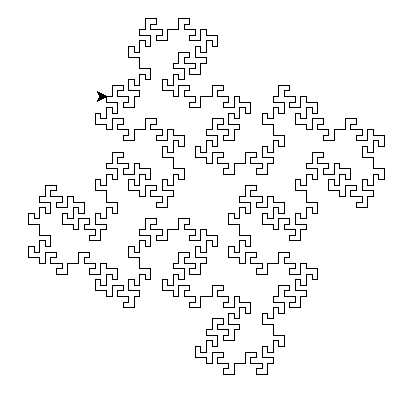
\includegraphics[width=0.333\textwidth]{kochtype16island} }
\caption{Koch type 1.6 island}
\label{kochtype16island}
\end{figure}


\end{itemize}

\item[Turn in:] Zip your four  grid programs and your
three island programs into a {\tt lab03 } folder and turn in on Canvas
before next Tuesday.

\end{description}
\end{document}

